\documentclass{ximera}

\newcommand{\RR}{\mathbb R}
\renewcommand{\d}{\,d}
\newcommand{\dd}[2][]{\frac{d #1}{d #2}}
\renewcommand{\l}{\ell}
\newcommand{\ddx}{\frac{d}{dx}}
\newcommand{\dfn}{\textbf}
\newcommand{\eval}[1]{\bigg[ #1 \bigg]}


\author{Bart Snapp}

\begin{document}
\begin{exercise}
  You are going to make a mathematical model of a \textit{torus} also
  known as a \textit{donut}.
  \begin{image}
  \includegraphics{donut.jpg}
  \end{image}
  Here is schematic (not to scale) diagram showing a cross-section
  found by cutting through the center of the donut with the plane
  $x=0$:
  \begin{image}
    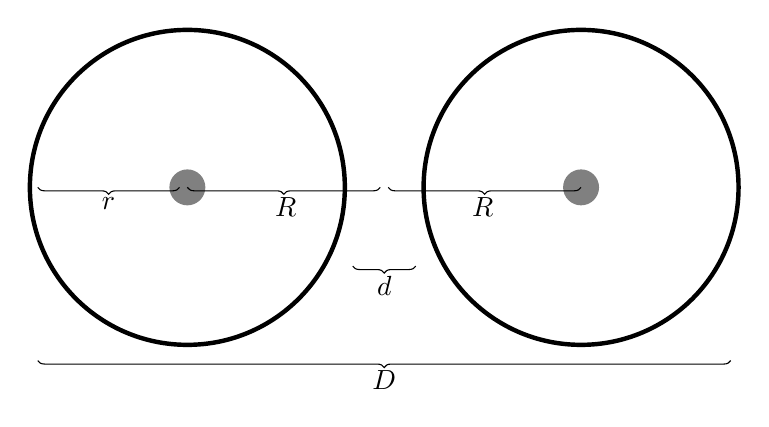
\begin{tikzpicture}
    \draw[ultra thick] (2.5,0) circle (2cm);
    \draw[ultra thick] (-2.5,0) circle (2cm);
    \draw[ultra thick,gray,fill] (2.5,0) circle (.2cm);
    \draw[ultra thick,gray,fill] (-2.5,0) circle (.2cm);
    \draw[decoration={brace,mirror},decorate,thin] (-.4,-1) -- (.4,-1);
    \draw[decoration={brace,mirror},decorate,thin] (-2.5,0) -- (-.05,0);
    \draw[decoration={brace},decorate,thin] (2.5,0) -- (.05,0);
    
    \draw[decoration={brace,mirror},decorate,thin] (-4.4,-2.2) -- (4.4,-2.2);
    \draw[decoration={brace,mirror},decorate,thin] (-4.4,0) -- (-2.6,0);

    \node[below] at (0,-2.2) {$D$};
    \node[below] at (0,-1) {$d$};
    \node[below] at (1.25,0) {$R$};
    \node[below] at (-1.25,0) {$R$};
    \node[below] at (-3.5,0) {$r$};    
  \end{tikzpicture}
  \end{image}
  Fill-in the values knowing that the donut should have an outer
  diameter of $6$ inches and a inner diameter (the hole) of $1$ inch.
  \[
  D=\answer{6}\qquad d=\answer{1}\qquad R=\answer{7/4} \qquad r=\answer{5/4}
  \]
  
  Imagine a circular curve in $\R^3$ that runs through the donut,
  shown in the diagram from the previous problem by the two ``dots.''
  \begin{image}
  \includegraphics{transdonut.jpg}
  \end{image}
  Give a formula for a vector-valued function $\vec{p}(t)$ that will
  draw a circle in the $(x,y)$-plane, centered at the origin, of radius
  $R$, as $t$ runs from $0$ to $2\pi$.
  \[
  \vec{p}(t) = \vector{\answer{(7/4)\cos(t)},\answer{(7/4)\sin(t)},\answer{0}}
  \]
  Compute $\utan(t)$, the function that will give the unit tangent
  vector for any value of $t$. \textbf{Simplify your answer.}
  \[
  \utan(t) = \vector{\answer{\sin(t)},\answer{\cos(t)},\answer{0}}
  \]
  Compute $\unormal(t)$, the function that will give the principal
  unit normal vector for any value of $t$. \textbf{Simplify your answer.}
  \[
  \unormal(t) =\vector{\answer{\cos(t)},\answer{\sin(t)},\answer{0}}
  \]
  Compute $\ubinormal(t)$, the function that will give the 
  unit binormal vector for any value of $t$. \textbf{Simplify your answer.}
  \begin{hint}
    Compute $\utan(t)\cross\unormal(t)$.
  \end{hint}
  \[
  \ubinormal(t) = \vector{\answer{0},\answer{0},\answer{1}}
  \]
  Give a vector-valued function $\vec{T}(s,t)$ of two variables $s$
  and $t$ that will plot the desired donut at $s$ runs from $0$ to
  $2\pi$ and as $t$ runs from $0$ to $2\pi$. 
  \[
  \vec{T}(s,t) = \vector{\answer{(7/4)\cos(t)+(5/4)\cos(t)\cos(s)},\answer{(7/4)\sin(t)+(5/4)\sin(t)\cos(s)},\answer{(5/4)\sin(s)}}
  \]
\end{exercise}
\end{document}
